\documentclass[12pt]{article}

\usepackage{amsmath}
\usepackage{unicode-math}
\usepackage{xltxtra}
\usepackage{xgreek}

\setmainfont{Liberation Serif}

\usepackage{tabularx}

\pagestyle{empty}

\usepackage{geometry}
 \geometry{a4paper, total={190mm,280mm}, left=10mm, top=10mm}

 \usepackage{graphicx}
 \graphicspath{ {images/} }

 \usepackage{wrapfig}

\begin{document}

\begin{table}
    \small
    \begin{tabularx}{\textwidth}{ c X r }
      \begin{tabular}{ l }
        Εισηγητής: Λόλας Κωνσταντίνος \\
        Επαναληπτικό: Όρια
      \end{tabular}
      & &
      \begin{tabular}{ r }
        Θεσσαλονίκη, 30 / 11 / 2023
      \end{tabular}
    \end{tabularx}
\end{table}

\part*{\centering{Διαγώνισμα Κατεύθυνση Γ Λυκείου}}

\section*{Θέμα Α}
  \noindent
  \begin{enumerate}
    \item \textbf{[Μονάδες 10]} Να διατυπώσετε το κριτήριο παρεμβολής
    \item \textbf{[Μονάδες 15]} Να χαρακτηρίσετε τις παρακάτω προτάσεις ως Σωστό ή Λάθος.
    \begin{enumerate}
        \item[α.] Αν υπάρχει το $\lim\limits_{x \to x_0}{ f(x) }>0$, τότε $f(x)>0$ κοντά στο $x_0$
        \item[β.] Αν $\lim\limits_{x \to x_0}{ f(x) }=+\infty$ ή $-\infty$, τότε $\lim\limits_{x \to x_0}{ \dfrac{1}{f(x)}=0 }$ 
        \item[γ.] Αν υπάρχει το $\lim\limits_{x \to x_0}{ \left(f(x)g(x)\right) }$, τότε κατ' ανάγκη υπάρχουν τα $\lim\limits_{x \to x_0}{ f(x) }$ και $\lim\limits_{x \to x_0}{ g(x) }$
        \item[δ.] Αν είναι $0<α<1$, τότε $\lim\limits_{x \to +\infty}{ α^x }=+\infty$
        \item[ε.] $\lim\limits_{x \to 0}{ \ln x }=1$ 
    \end{enumerate}
  \end{enumerate}

\section*{Θέμα Β}
  \noindent
  Στο σχήμα δίνεται η γραφική παράσταση μιας συνάρτησης $f$ που είναι ορισμένη στο $\mathbb{R}$. Να βρείτε (αν υπάρχουν) τα παρακάτω όρια.
  \begin{figure}[h]
    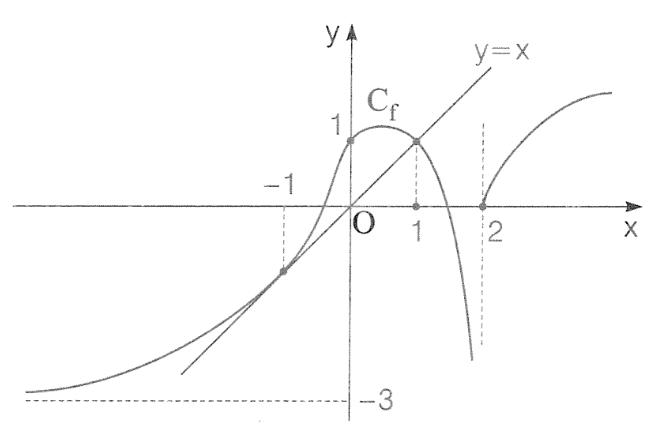
\includegraphics[width=8cm]{oriatest.png}
    \centering
    \end{figure}
  \begin{enumerate}
    \item \textbf{[Μονάδες 5]} $\lim\limits_{x \to -\infty}{ f(x) }$
    \item \textbf{[Μονάδες 5]} $\lim\limits_{x \to -1}{ \dfrac{x}{f(x)-x} }$
    \item \textbf{[Μονάδες 5]} $\lim\limits_{x \to 0}{ \dfrac{f(x)}{e^{|x|}-1} }$
    \item \textbf{[Μονάδες 5]} $\lim\limits_{x \to 1}{ \dfrac{x}{f(x)-x} }$
    \item \textbf{[Μονάδες 5]} $\lim\limits_{x \to 2}{ \dfrac{\sqrt{2-x}}{f(x)} }$
  \end{enumerate}
  Για τα όρια που δεν υπάρχουν να δικαιολογήσετε την απάντησή σας
  %\vspace{7\baselineskip}

\section*{Θέμα Γ}
  \noindent
  Δίνεται η συνάρτηση $f(x)=x^2+1$. Να βρείτε τα όρια:
  \begin{enumerate}
    \item \textbf{[Μονάδες 5]} $\lim\limits_{x \to 1}{ \dfrac{f(x)+x-3}{x^3-1} }$
    \item \textbf{[Μονάδες 5]} $\lim\limits_{x \to 1^+}{ \dfrac{f(x)}{x-1} }$
    \item \textbf{[Μονάδες 5]} $\lim\limits_{x \to +\infty}{ \left( \sqrt{f(x)}-x \right)}$   
    \item \textbf{[Μονάδες 5]} $\lim\limits_{x \to +\infty}{ \left( f(x)+ημx \right)}$
    \item \textbf{[Μονάδες 5]} $\lim\limits_{x \to +\infty}{ \dfrac{συνx}{f(x)}}$
  \end{enumerate}

  \section*{Θέμα Δ}
    \noindent
    Δίνονται οι συναρτήσεις
    $$f(x)=\dfrac{\ln x}{x} \text{ και } g(x)=xe^{-\frac{1}{x}}$$
    Να βρείτε τα όρια
    \begin{enumerate}
        \item \textbf{[Μονάδες 6]} $\lim\limits_{x \to 0}{ f(x)}$
        \item \textbf{[Μονάδες 6]} $\lim\limits_{x \to 0}{ \dfrac{xf(x)}{ημx}}$
        \item \textbf{[Μονάδες 6]} $\lim\limits_{x \to 0^+}{ g(x)}$
        \item \textbf{[Μονάδες 7]} $\lim\limits_{x \to 0^+}{ f\left(g(x)\right)}$
    \end{enumerate}

\vspace{2\baselineskip}

\part*{\centering{Καλή επιτυχία}}

\end{document}
